%% ****** Start of file apstemplate.tex ****** %
%%
%%
%%   This file is part of the APS files in the REVTeX 4.2 distribution.
%%   Version 4.2a of REVTeX, January, 2015
%%
%%
%%   Copyright (c) 2015 The American Physical Society.
%%
%%   See the REVTeX 4 README file for restrictions and more information.
%%
%
% This is a template for producing manuscripts for use with REVTEX 4.2
% Copy this file to another name and then work on that file.
% That way, you always have this original template file to use.
%
% Group addresses by affiliation; use superscriptaddress for long
% author lists, or if there are many overlapping affiliations.
% For Phys. Rev. appearance, change preprint to twocolumn.
% Choose pra, prb, prc, prd, pre, prl, prstab, prstper, or rmp for journal
%  Add 'draft' option to mark overfull boxes with black boxes
%  Add 'showkeys' option to make keywords appear
\documentclass[aps,prx,preprint,groupedaddress]{revtex4-2}
\usepackage{graphicx}
\usepackage{amsmath}
%\documentclass[aps,prl,preprint,superscriptaddress]{revtex4-2}
%\documentclass[aps,prl,reprint,groupedaddress]{revtex4-2}
% You should use BibTeX and apsrev.bst for references
% Choosing a journal automatically selects the correct APS
% BibTeX style file (bst file), so only uncomment the line
% below if necessary.
%\bibliographystyle{apsrev4-2}

\begin{document}

% Use the \preprint command to place your local institutional report
% number in the upper righthand corner of the title page in preprint mode.
% Multiple \preprint commands are allowed.
% Use the 'preprintnumbers' class option to override journal defaults
% to display numbers if necessary
%\preprint{}

%Title of paper
\title{Entanglement features in the Kondo Model}
%Holographic distillation of topological order in a correlated quantum liquid}

% repeat the \author .. \affiliation  etc. as needed
% \email, \thanks, \homepage, \altaffiliation all apply to the current
% author. Explanatory text should go in the []'s, actual e-mail
% address or url should go in the {}'s for \email and \homepage.
% Please use the appropriate macro foreach each type of information

% \affiliation command applies to all authors since the last
% \affiliation command. The \affiliation command should follow the
% other information
% \affiliation can be followed by \email, \homepage, \thanks as well.
\author{Anirban Mukherjee}
\email[]{am14rs016@iiserkol.ac.in}
\author{N.S. Vidhyadhiraja}
\email[]{raja@jncasr.in}
\author{Siddhartha Lal}
\email[]{slal@iiserkol.ac.in}
\author{Arghya Tarapdher}
\email[]{arghya@phy.kgp.ernet.in}

%\homepage[]{Your web page}
%\thanks{}
%\altaffiliation{}
\affiliation{Department of Physical Sciences, IISER Kolkata}

%Collaboration name if desired (requires use of superscriptaddress
%option in \documentclass). \noaffiliation is required (may also be
%used with the \author command).
%\collaboration can be followed by \email, \homepage, \thanks as well.
%\collaboration{}
%\noaffiliation

\date{\today}

\begin{abstract}
abstract..
% insert abstract here
\end{abstract}
% insert suggested keywords - APS authors don't need to do this
%\keywords{}

%\maketitle must follow title, authors, abstract, and keywords
\maketitle
%
%% body of paper here - Use proper section commands
%% References should be done using the \cite, \ref, and \label commands
%\section{Motivation}
%The key feature of the Kondo screening cloud is the entanglement content between a magnetic impurity and conduction electrons in the vicinity of the Fermi surface. A recent work Phys. Rev. Lett. 120, 146801 (2018) shows that the entanglement content is related to electronic conductivity. In many body systems entanglement entropy scaling shows distinct features for gapped as against gapless phases Phys. Rev. Lett. (2007), arxiv:2003.06118 (2020).  Are there any observable entanglement RG scaling features with regards to formation of the Kondo cloud? Our  URG procedure mitigates fermion exchange signatures , i.e. it functions as a decoder circuit comprising a error correcting code leading to an emergent subspace where an electronic cloud entangles with the Kondo spin. In this work we want to study the interplay fermion exchange signatures, many particle entanglement, and quantum transport observables like conductivity, shot noise, spectral function etc.\\
%\par\noindent
%\textbf{List of things we can do}
%\par\noindent
%\begin{enumerate}
%\item[1.]We can start with the Heisenberg Kondo Hamiltonian with isotropic Fermi surface of the Fermi liquid and obtain the URG flow in the space of Hamiltonians arranged from UV to IR. From the IR fixed points obtained in the antiferromagnetic side of the Kondo model we can compute the effective Hamiltonian and the eigenstates.
%\item[2.]Our experience suggests that the effective Hamiltonian in the strong coupling regime on the antiferromagnetic side will be of the pseudospin kind. By reversing the RG flow we can tomographically create the many body states at UV, by re-entangling the high energy electronic states with their IR counterparts. This allows realization of an entanglement renormalization group and altogether comprise the construction of the EHM tensor network.
%\item[3.]In the construction of the entanglement RG flow we can study the effect of fermion exchange signatures in the entanglement entropy, mutual information (MI) flow. We can also study the Ryu-Takayanagi entropy bound, emergent holographic spacetime generated from MI. Can this entanglement features witness the entanglement phase transition between the ferromagnetic and antiferromagnetic side of the Kondo model?
%\item[4.]We can extract the reduced density matrix comprising the HIlbert space associated with the Fermi surface (FS) and the Kondo Impurity (KI). We can study the RG dynamics of MI content between the FS and the KI, does this show the formation of the Kondo cloud? Does the fermion exchange signs have observable effects in the entanglement scaling flow towards the Kondo cloud?
%\item[5.]In the case when the Kondo cloud is formed can we confirm Martin’s sum rule, i.e. the reduction in Luttinger’s sum by the no. of electronic states added to the KI. This implies that the ferromagnetic to antiferromagnetic transition is a topological transition. How does this coincide with our understanding of the entanglement phase transition?
%\item[6.]Finally we can study the holographic renormalization of the quantum geometric tensor for the Fermi surface and KI HIlbert space, this will surely be a witness to the formation of the Kondo cloud.
%\item[7.]Show quantum advantage in the kondo cloud for error correction. But it requires a bit more study of the current plan. Especially the entanglement scaling features fermion sign issues. Then we can understand how they get error corrected upon scaling, and eventually form the cloud, i.e., How fermion sign issues are resolved resulting in the formation of Kondo cloud. This could be used in a proposal for quantum error correction and an equivalent machine learning protocol.
%\item[8.]Can we perform a gauge theoretic construction of the local quantum liquid generated by isolating the Kondo impurity via tracing out its degree of freedom?
%\end{enumerate}
\section{Introduction}
\par\noindent
Literature survey...\\
\emph{Motivation for the work} In the antiferromagnetic side a Kondo cloud is formed via the entanglement between the impurity spin and conduction electrons. On the otherhand in the ferromagnetic side the impurity spin disentangles from the conduction electrons. In the present work we want to study the interplay between electronic correlation in the Fermi surface neighbourhood and fermion exchange
signs in shaping the entanglement between the Kondo cloud and the impurity spin.
For the study we will use a unitary renormalization group (URG) theory for the Kondo model. Using a combination of entangled based and Green function based measures we will unravel the quantum correlation of Kondo cloud.
\section{The Model}
The Kondo model\cite{kondo1964resistance,anderson1970poor} describes the coupling between a magnetic quantum impurity localized in real space with a conduction electron bath,
\begin{eqnarray}
\hat{H} = \sum_{\mathbf{k}\sigma}\epsilon_{\mathbf{k}}\hat{n}_{\mathbf{k}\sigma}+\frac{J}{2}\sum_{\mathbf{k},\mathbf{k}'}\mathbf{S}\cdot c^{\dagger}_{\mathbf{k}\alpha}\boldsymbol{\sigma}_{\alpha\beta}c_{\mathbf{k}'\beta}~.\label{KondoH}
\end{eqnarray}
Here we consider a 2d electronic bath $\epsilon_{\mathbf{k}}=-2t(\cos k_{x}+\cos k_{y})$ with the Fermi energy $E_{F}=\mu$. $J$ is the Kondo scattering coupling between the impurity and the conduction electrons. An important feature of the Kondo coupling is the two different classes of scattering processes, one involving spin flip $c^{\dagger}_{\mathbf{k}\uparrow}c_{\mathbf{k}'\downarrow}+h.c.$ another not involving spin flip. In the antiferromagnetic regime $J>0$ the spin flip scattering processes generates quantum entanglement between the impurity spin and the Kondo cloud resultingly screening the impurity.

\section{URG theory for the Kondo Model}
\par\noindent
We construct a unitary RG theory for the Kondo model, electronic states from the bath are stepwise disentangled starting with the highest energy electrons eventually scaling towards the Fermi surface. The electronic states are labelled in terms of the normal distance $\Lambda$ from the Fermi surface and the orientation unit vectors (Fig.\ref{FSgeom})$\hat{s}$: $\mathbf{k}_{\Lambda\hat{s}}=\mathbf{k}_{F}(\hat{s})+\Lambda\hat{s}$ where $\hat{s}=\frac{\nabla\epsilon_{\mathbf{k}}}{|\nabla\epsilon_{\mathbf{k}}|}|_{\epsilon_{\mathbf{k}}=E_{F}}$. The states are labelled as
$|j,l,\sigma\rangle = |\mathbf{k}_{\Lambda_{j}\hat{s}},\sigma\rangle, l:=(\hat{s}_{m},\sigma)$. 
\begin{figure}
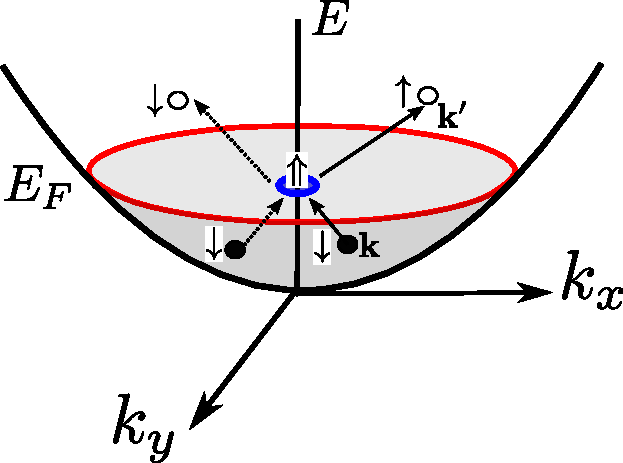
\includegraphics[scale=0.75]{kondoSetup.pdf}
\caption{The Kondo model is composed of a two dimensional conduction electron bath (Fermi liquid) coupled to a magnetic impurity via spin flip(solid)/non spin flip(dashed) scattering processes.}
\end{figure}
\begin{figure*}
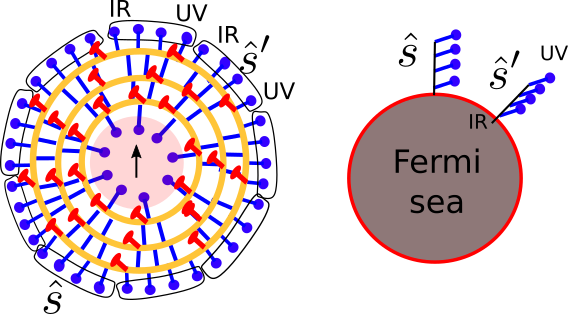
\includegraphics[scale=1]{TNKondo.png}
\caption{Figure in the left shows a tensor network representation of the Kondo RG with  8 Fermi surface patches. The 32 blue nodes represents the 8 (for 8 $\hat{s}$) sets of 4(along a given normal $\hat{s}$) electronic states (qubits).  arranged from UV to IR (see figure in the right). The yellow circular block represents the unitary gate that disentangles at each RG step 8 electronic qubits at UV. The red nodes represents the disentangled qubits comprising the bulk of the tensor network. At the IR bulk of the tensor network the pink circle represents the Kondo cloud coupling with the spin vector (up arrow).} \label{KondoTN}
\end{figure*}




The $\Lambda$'s are arranged as follows: $\Lambda_{N}>\Lambda_{N-1}>\ldots>0$, where the electronic states farthest from Fermi surface $\Lambda_{N}$ is disentangled first, eventually scaling towards the Fermi surface. This leads to the Hamiltonian flow equation,
\begin{equation}
\centering
H_{(j-1)}=U_{(j)}H_{(j)}U^{\dagger}_{(j)}~.
\end{equation}
where the unitary operation $U_{(j)}$ is the unitary map. $U_{(j)}$ disentangles all the electronic states $\mathbf{k}_{\Lambda_{j}\hat{s}_{m}},\sigma$ on the isogeometric curve and has the form\cite{anirbanmotti},
\begin{equation}
\centering U_{(j)}=\prod_{l}U_{j,l}, U_{j,l}=\frac{1}{\sqrt{2}}[1+\eta_{j,l}-\eta^{\dagger}_{j,l}],
\end{equation}
where $\eta_{j,l}$ are electron hole transition operators following the algebra,
\begin{equation}
\lbrace\eta_{j,l},\eta_{j,l}^{\dagger}\rbrace=1, \left[\eta_{j,l},\eta_{j,l}^{\dagger}\right]=1~.
\end{equation}
The transition operator in terms of the diagonal $H^{D}$ and off-diagonal parts of the Hamiltonian $H^{X}$ has the form,  
\begin{eqnarray}
\eta_{j,l}&=&Tr_{j,l}(c^{\dagger}_{j,l}H_{j,l})c_{j,l}\frac{1}{\hat{\omega}_{j,l}-Tr_{j,l}(H_{j,l}^{D}\hat{n}_{j,l})\hat{n}_{j,l}}.~~\label{e-TransOp}
\end{eqnarray}
In the numerator the operator $Tr_{j,l}(c^{\dagger}_{j,l}H_{j,l})c_{j,l}+h.c.$ is composed of all possible scattering vertices that modify the configuration of the electronic state $|j,l\rangle$. The generic forms of $H^{D}_{j,l}$, $H^{X}_{j,l}$ are as follows,
\begin{eqnarray}
H^{D}_{j,l}&=&\sum_{\Lambda\hat{s},\sigma}\epsilon^{j,l}\hat{n}_{\mathbf{k}_{\Lambda\hat{s}},\sigma}+\sum_{\alpha}\Gamma_{\alpha}^{4,(j,l)}\hat{n}_{\mathbf{k}\sigma}\hat{n}_{\mathbf{k}'\sigma'}+\sum_{\beta}\Gamma_{\beta}^{8,(j,l)}\hat{n}_{\mathbf{k}\sigma}\hat{n}_{\mathbf{k}'\sigma'}(1-\hat{n}_{\mathbf{k}''\sigma''})+\ldots\nonumber\\
H^{X}_{j,l}&=&\sum_{\alpha}\Gamma_{\alpha}^{2}c^{\dagger}_{\mathbf{k}\sigma}c_{\mathbf{k}'\sigma'}+\sum_{\beta}\Gamma_{\beta}^{4}c^{\dagger}_{\mathbf{k}\sigma}c^{\dagger}_{\mathbf{k}'\sigma'}c_{\mathbf{k}_{1}'\sigma_{1}'}c_{\mathbf{k}_{1}\sigma_{1}}+\sum_{\beta}\Gamma_{\beta}^{6}c^{\dagger}_{\mathbf{k}\sigma}c^{\dagger}_{\mathbf{k}'\sigma'}c_{\mathbf{k}_{1}'\sigma_{1}'}c_{\mathbf{k}_{1}\sigma_{1}}\ldots~~~
\end{eqnarray}
The operator $\hat{\omega}_{j,l}$ accounts for the quantum fluctuation arising from the non commutivity between different parts of the renormalized Hamiltonian and has the form,\cite{anirbanurg1}
\begin{eqnarray}
\hat{\omega}_{j,l}&=&H^{D}_{j,l}+H^{X}_{j,l}-H^{X}_{j,l-1}~.\label{qfOp}
\end{eqnarray}
Upon disentangling electronic states $\hat{s},\sigma$ along a isogeometric curve at distance $\Lambda_{j}$ the effective Hamiltonians $H_{j,l}$ are generated,
\begin{eqnarray}
H_{j,l}=\prod_{m=1}^{l}U_{j,m}H_{(j)}[\prod_{m=1}^{l}U_{j,l}]^{\dagger}~.
\end{eqnarray}
After having disentangled all the electronic states $2n_{j}$ on the isogeometric curve the effective Hamiltonian $H_{j,2n_{j}+1}=H_{(j-1)}$ for the next RG step is obtained. Disentangling multiple qubits succesively in a given momentum shell at distance $\Lambda_{j}$ from FS leads to renormalized contribution from one and higher  particle correlated tangential scattering process. Accounting for the leading tangential scattering processes and other momentum transfer processes along normal $\hat{s}$ the renormalized Hamiltonian has the form,
\begin{eqnarray}
H_{(j-1)}&=&Tr_{j,(1,\ldots,2n_{j})}(H_{(j)})+\sum_{l=1}^{2n_{j}}\lbrace c^{\dagger}_{j,l}Tr_{j,l}(H_{(j)}c_{j,l}),\eta_{j,l}\rbrace\tau_{j,l}~.~~~\label{HRG}
\end{eqnarray}
Here $2n_{j}$ are the number of electronic states on the curve at distance $\Lambda_{j}$.
\section{Results}
\par\noindent
The unitary RG process generates the effective Hamiltonian's $\hat{H}_{(j)}(\omega)$'s for various eigen directions $|\Phi(\omega)\rangle$
of the $\hat{\omega}$ operator. Note the associated eigenvalue $\omega$ identifies a subspectrum in the interacting many body eigenspace. The form of $\hat{H}_{(j)}(\omega)$ is given by,
\begin{eqnarray}
\hat{H}_{(j)}(\omega) &=& \sum_{j,l,\sigma}\epsilon_{j,l}\hat{n}_{j,l}+\frac{J^{(j)}(\omega)}{2}\sum_{\substack{j_{1},j_{2}<j,\\ m,m'}}\mathbf{S}\cdot c^{\dagger}_{j_{1},\hat{s}_{m},\alpha}\boldsymbol{\sigma}_{\alpha\beta}c_{j_{2},\hat{s}_{m'},\beta}+\sum^{j,n_{j}}_{\substack{a=N,\\ m=1}}J^{(a)}S^{z}s^{z}_{a,\hat{s},m},
\end{eqnarray}
where  $s^{z}_{l,\hat{s},m}=\frac{1}{2}(\hat{n}_{l,\hat{s}_{m},\uparrow}-\hat{n}_{l,\hat{s}_{m},\downarrow})$. The Kondo coupling RG equation for the RG steps(Appendix\ref{Appendix-A}) has the form,
\begin{eqnarray}
\frac{\Delta J^{(j)}(\omega)}{\Delta\log\frac{\Lambda{j}}{\Lambda_{0}}}=\frac{2n_{j}(J^{(j)})^{2}\left[(\frac{\epsilon_{j}}{2}-\omega)\right]}{(\frac{\epsilon_{j}}{2}-\omega)^{2}-\frac{\left(J^{(j)}\right)^{2}}{16}}\label{RGeqn}
\end{eqnarray}
Note the denominator $\Delta\log\frac{\Lambda{j}}{\Lambda_{0}} =1$ for the RG scale parameterization $\Lambda_{j}=\Lambda_{0}\exp(-j)$. We redefine Kondo coupling as a dimensionless parameter,
\begin{eqnarray}
K^{(j)}=\frac{J^{(j)}}{\frac{\epsilon_{j}}{2}-\omega}~,\label{reparametrization}
\end{eqnarray} 
We operate in the regime $\frac{\epsilon_{j}}{2}>\omega$. In order to obtain a continuum RG equation we approximate the dispersion  $\epsilon_{j}=(2m)^{-1}(\hbar k_{F}+v_{F}\Lambda)^{2}-\hbar^{2}k_{F}^{2}\approx \hbar v_{F}\Lambda$ for $\Lambda<\Lambda_{0}$,
\begin{eqnarray}
\frac{d K}{d\log\frac{\Lambda}{\Lambda_{0}}}=\left(1+\frac{\omega}{\hbar v_{F}\Lambda}-\omega\right)K+\frac{n(\Lambda)K^{2}}{1-\frac{K^{2}}{16}}
\end{eqnarray}
Upon approaching the Fermi surface $\Lambda_{j}\to 0$ therefore $\left(1-\frac{\omega}{\omega-\hbar v_{F}\Lambda}\right)\to 0$ for $\omega\to 0-$  and $n(\Lambda)$ can be replaced by no. of states on the Fermi surface $n(0)$, leading to 
\begin{eqnarray}
\frac{d K}{d\log\frac{\Lambda}{\Lambda_{0}}}=\frac{n(0)K^{2}}{1-\frac{K^{2}}{16}}
\end{eqnarray}
\begin{figure}[h!]
\centering
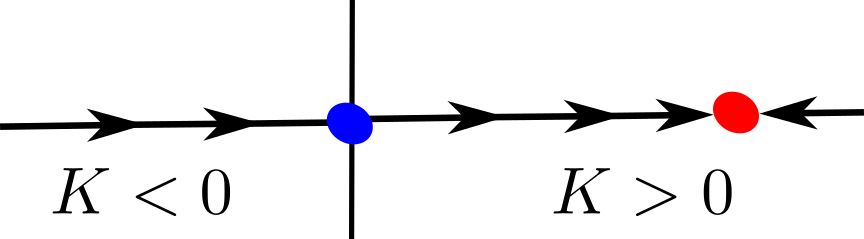
\includegraphics[scale=0.6]{Kondo.png}
\caption{Schematic RG phase diagram. Red dot represents intermediate coupling fixed point. Blue dot is the critical fixed point.} 
\end{figure}
\begin{figure}
\centering
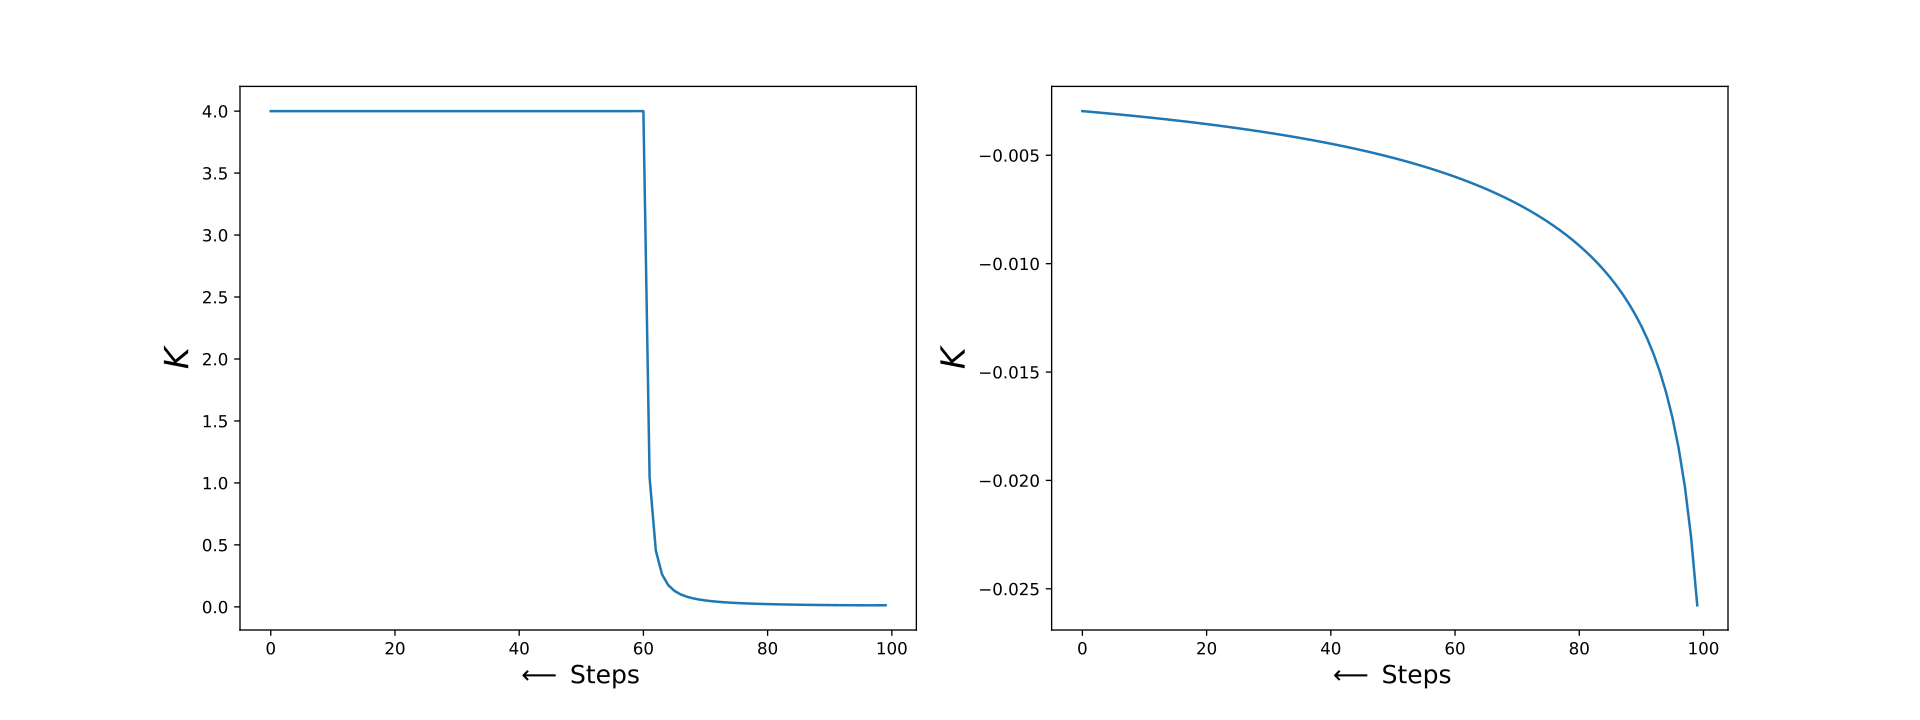
\includegraphics[width=\textwidth]{RG_Flow.png}
\caption{Renormalized dimensionless Kondo coupling $K$ with RG steps ($\log\Lambda_{j}/\Lambda_{0}$), left panel:$K>0$, right panel: $K<0$.} 
\end{figure}
We observe two important aspects of the RG equation: for $K<<1$ the RG equation reduces to the one loop form, $\frac{d K}{d\log\frac{\Lambda}{\Lambda_{0}}}=K^{2}$\cite{anderson1970poor}. On the otherhand the nonperturbative form of flow equations shows the presence of intermediate coupling fixed points $K^{*}=4$ in the antiferromagnetic regime $K>0$.
Upon integrating the RG equation and using the fixed point value $K^{*}=4$ we obtain the energy scale,
\begin{eqnarray}
&&\frac{1}{K_{0}}-\frac{1}{2}+\frac{K_{0}}{16}=-n(0)\log\frac{\Lambda}{\Lambda_{0}}\nonumber\\
&&\Lambda=\Lambda_{0}\exp\left(\frac{1}{2n(0)}-\frac{1}{n(0)K_{0}}-\frac{K_{0}}{n(0)16}\right)\label{gap function}
\end{eqnarray}
\par\noindent
At the IR fixed point in the AF regime the effective Hamiltonian is given by,
\begin{eqnarray}
H^{*}=\sum_{|\Lambda|<\Lambda^{*}}\hbar v_{F}\Lambda\hat{n}_{\Lambda,\hat{s},\sigma}+\frac{J^{*}}{2}\sum_{\substack{j_{1},j_{2}<j^{*},\\ m,m'}}\mathbf{S}\cdot c^{\dagger}_{j_{1},\hat{s}_{m},\alpha}\boldsymbol{\sigma}_{\alpha\beta}c_{j_{2},\hat{s}_{m'},\beta}+\sum_{j'=N,m=1}^{j^{*},n_{j'}}J^{j'}S^{z}s^{z}_{j',m}\label{fixedPointHam}
\end{eqnarray} 
We can now extract a zero mode from the above Hamiltonian that captures the low energy theory near the Fermi surface,
\begin{eqnarray}
H^{*}_{K}&=&\frac{1}{N}\sum_{|\Lambda|<\Lambda^{*}}\hbar v_{F}\Lambda\sum_{|\Lambda|<\Lambda^{*}}\hat{n}_{\Lambda,\hat{s},\sigma}+\frac{J^{*}}{2}\sum_{\substack{j_{1},j_{2}<j^{*},\\ m,m'}}\mathbf{S}\cdot c^{\dagger}_{j_{1},\hat{s}_{m},\alpha}\boldsymbol{\sigma}_{\alpha\beta}c_{j_{2},\hat{s}_{m'},\beta}+\sum_{j'=N,m=1}^{j,n_{j'}}J^{j'}S^{z}s^{z}_{j',m}\nonumber\\
		&=&\frac{J^{*}}{2}\sum_{\substack{j_{1},j_{2}<j^{*},\\ m,m'}}\mathbf{S}\cdot c^{\dagger}_{j_{1},\hat{s}_{m},\alpha}\boldsymbol{\sigma}_{\alpha\beta}c_{j_{2},\hat{s}_{m'},\beta}+\sum_{j'=N,m=1}^{j^{*},n_{j'}}J^{j'}S^{z}s^{z}_{j',m}~.
\end{eqnarray}
Indeed we observe that the zero mode Hamiltonian at the IR fixed point is responsible for the formation of the singlet ground state.
\begin{equation}
|\Psi*\rangle=\frac{1}{\sqrt{2}}\left[|\uparrow\rangle\sum_{\Lambda,\hat{s}}|1_{\Lambda,\hat{s},\downarrow}\rangle\otimes_{\Lambda'\neq\Lambda,\hat{s}'\neq \hat{s}}|\Lambda',\hat{s}'\rangle-|\downarrow\rangle\sum_{\Lambda,\hat{s}}|1_{\Lambda,\hat{s},\uparrow}\rangle\otimes_{\Lambda'\neq\Lambda,\hat{s}'\neq \hat{s}}|\Lambda',\hat{s}'\rangle\right]
\end{equation}
\subsection{Variation of the Kondo cloud size $\xi$ and effective Kondo coupling $J^{*}$ as function of bare coupling $J_{0}$}
All plots below are obtained for momentum space grid $100\times 100$ and with RG scale factor ($b=0.9999$) $\Lambda_{j}=b\Lambda_{j+1}$. The $E_{F}$ for the 2d tight binding band $-W/2<E_{k}=-2t(\cos k_{x}+\cos k_{y})<W/2$ ($W=4t$) is chosen at $E_{F}=-3.8t$. 
\begin{figure}
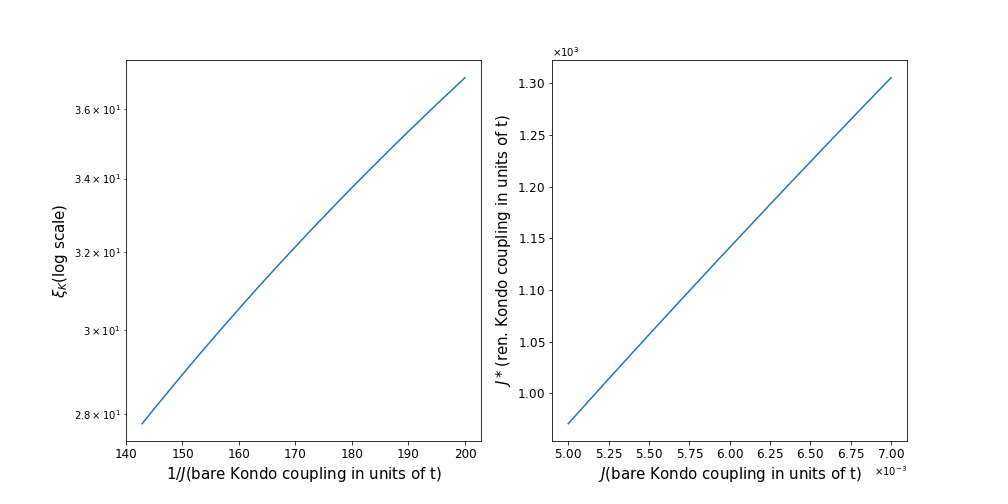
\includegraphics[width=\textwidth]{KondoRegime1.png}
\caption{Left panel: Kondo cloud length $\xi$ in log scale (y-axis) vs. $1/J_{0}$ (x-axis), right panel: renormalized Kondo coupling $J^{*}$ vs. $J_{0}$, for $5\times 10^{-3}t<J_{0}<7\times 10^{-3}t$.}
\end{figure}
\begin{figure}
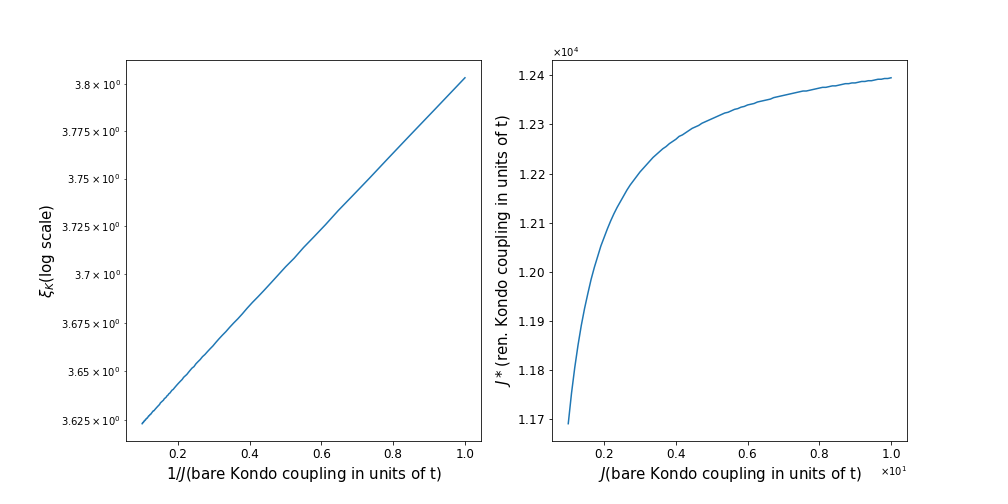
\includegraphics[width=\textwidth]{KondoRegime3.png}
\caption{Left panel: Kondo cloud length $\xi$ in log scale (y-axis) vs. $1/J_{0}$ (x-axis), right panel: renormalized Kondo coupling $J^{*}$ vs. $J_{0}$, for $t<J_{0}<7\times 10^{-3}t$.}
\end{figure}
\begin{figure}
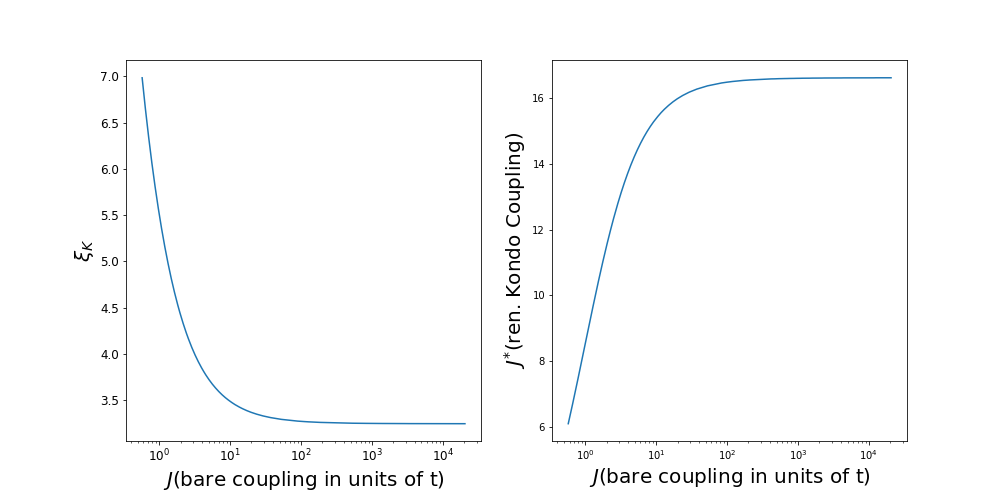
\includegraphics[width=\textwidth]{KondoComplete.png}
\caption{Left panel: Kondo cloud length $\xi$ vs. $J_{0}$ (x-axis in log scale) in , right panel: renormalized Kondo coupling $J^{*}$ vs. $J_{0}$. $J_{0}$ is chosen as $4.9\times 10^{-3}\times(1.02656)^{n}$ and $1<n<1000$.}
\end{figure}
\section{Impurity spin susceptibility and specific heat calculation for the Kondo Hamiltonian}
The effective Hamiltonian obtained at the IR fixed point eq.\eqref{fixedPointHam} commutes with the z-component of the net spin vector,
\begin{eqnarray}
S^{z}_{tot}=S^{z}+\sum_{\substack{\Lambda,\Lambda'<\Lambda^{*},\\ m,m'\\\alpha,\beta}}c^{\dagger}_{\Lambda,\hat{s}_{m},\alpha}\frac{\sigma_{\alpha\beta}^{z}}{2}c_{\Lambda',\hat{s}_{m'},\beta}+\sum_{\Lambda\geq \Lambda^{*},m}S^{z}s^{z}_{\Lambda,m},~~~ s^{z}_{\Lambda,m}=\frac{1}{2}\left(\hat{n}_{\Lambda,\hat{s}_{m},\uparrow}-\hat{n}_{\Lambda,\hat{s}_{m},\downarrow}\right)~.~~~
\end{eqnarray}
Let us defined the fourier transform of the electronic states for $\Lambda<\Lambda^{*}$,
\begin{eqnarray}
c^{\dagger}_{\Lambda,\hat{s}_{m},\sigma}=\frac{1}{\sqrt{L^{*}}}\sum_{\mathbf{r}}e^{i\mathbf{k}_{\Lambda\hat{s}_{m}}\cdot\mathbf{r}}d^{\dagger}_{\mathbf{r}\sigma}
\end{eqnarray}
\begin{eqnarray}
\sum_{\Lambda,\Lambda',m,m'} c^{\dagger}_{\Lambda,\hat{s}_{m},\alpha}\frac{\boldsymbol{\sigma}_{\alpha\beta}}{2}c_{\Lambda',\hat{s}_{m'},\beta}=\sum_{\mathbf{r},\mathbf{r}'}e^{i\mathbf{k}_{\Lambda\hat{s}_{m}}\cdot\mathbf{r}-i\mathbf{k}_{\Lambda'\hat{s}_{m'}}\cdot\mathbf{r}'}d^{\dagger}_{\mathbf{r}\alpha}\frac{\boldsymbol{\sigma}_{\alpha\beta}}{2}\mathbf{d}_{\mathbf{r}'\beta}=d^{\dagger}_{0,\alpha}\frac{\boldsymbol{\sigma}_{\alpha\beta}}{2}d_{0,\beta}
\end{eqnarray}
\begin{eqnarray}
\left[\sum_{\mathbf{k}\sigma'}\epsilon_{\mathbf{k}}\hat{n}_{\mathbf{k}\sigma'},\sum_{\mathbf{k}_{1},\mathbf{k}_{2}}\sigma c^{\dagger}_{\mathbf{k}_{1}\sigma}c_{\mathbf{k}_{2}\sigma}\right]=\delta_{\sigma\sigma'}\delta_{\mathbf{k}_{1},\mathbf{k}}\sigma(\left[\hat{n}_{\mathbf{k}\sigma},c^{\dagger}_{\mathbf{k}\sigma}c_{\mathbf{k}'\sigma}\right]+\left[\hat{n}_{\mathbf{k}\sigma},c^{\dagger}_{\mathbf{k}'\sigma}c_{\mathbf{k}\sigma}\right])\nonumber\\
c^{\dagger}_{\mathbf{k}\sigma}c_{\mathbf{k}'\sigma}(1-\hat{n}_{\mathbf{k}\sigma})-
\end{eqnarray}
\begin{eqnarray}
[H^{*},S^{z}_{tot}]=0
\end{eqnarray}
The spin susceptibility originating purely from the impurity at the IR fixed originating simply from the impurity can be defined as,
\begin{equation}
\chi(T)=\frac{1}{kT}\left[\frac{Tr((S^{z}_{tot})^{2}\exp(-H^{*}(J^{*})/kT)}{Tr(\exp(-H^{*}(J^{*})/kT))}-\left(\frac{Tr((S^{z}_{tot})^{2}\exp(-H^{*}(0)/kT)}{Tr(\exp(-H^{*}(0)/kT))}-\frac{1}{4}\right)\right]
\end{equation}
Since the eigenvalues of $S^{z}_{tot}$ are good quantum nos for the eigenstates of $H^{*}$ we can use those states to obtain these quantity. Similar thing can be done for the specific heat. The second term in the above expression cancels of the contribution coming to susceptibility from conduction electrons at $J^{*}=0$. The final term $1/4$ cancels of the impurity susceptibility from $J^{*}=0$ term. This prescription is due to Wilson \cite{wilson1975renormalization}. The eigenstates and eigenvalues of $H^{*}$ is given by,
\section{Tensor network representation of the Kondo URG program}
In this section we present the tensor network representation of the URG program\cite{anirbanurg1,mukherjee2020}. The yellow blocks represent the complete U transformation $U_{(j)}$ for a given RG step that is composed of $U_{j,l}$ here individual $U_{j,l}$ disentangles one electronic state $\mathbf{k}_{\Lambda\hat{s}},\sigma$. The wavefunction $|\Psi^{*}\rangle$ comprises the IR bulk of the tensor network. The yellow layers are arranged along the RG direction. 
\begin{figure}
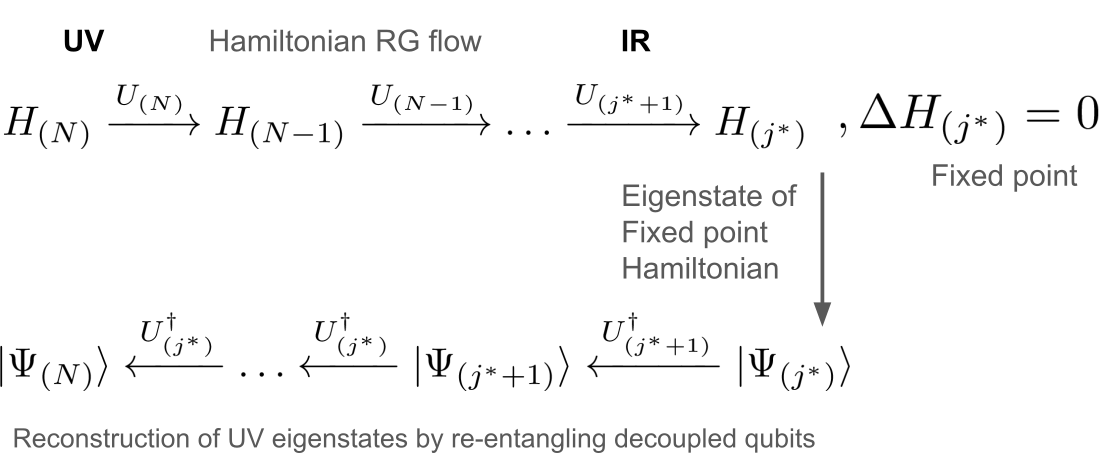
\includegraphics[width=\textwidth]{flowChart.png}
\caption{The first line represent the Hamiltonian RG flow via the unitary maps. Upon reaching the Kondo IR fixed point, reverse RG will re-entangled decoupled electronic states with the Kondo singlet. This will result in generation of the many body eigenstates at UV.}  \label{eigenUV}
\end{figure}
The tensor network Fig.\ref{KondoTN} is composed of yellow layers that lead to a holographic arrangement of eigenstates from UV to IR. From the singlet state obtained at RG fixed point we can perform the inverse unitary map to regenerate the entanglement with UV degrees of freedom Fig.\eqref{eigenUV}. This enables udsd to obtain the complete form of the two point retarded green function along the RG flow direction (RG time)$\tau_{j}=1/v_{F}\Lambda_{j}$,
\begin{eqnarray}
G(\mathbf{k}\sigma,\tau;\mathbf{k}'\sigma',\tau')=\Theta(\tau-\tau')\langle\Psi_{0}|\lbrace c_{\mathbf{k}\sigma}(\tau)c^{\dagger}_{\mathbf{k}'\sigma'}(\tau')\rbrace|\Psi_{0}\rangle
\end{eqnarray} 
where $|\Psi_{0}\rangle= U^{\dagger}_{N}\ldots U^{\dagger}_{j^{*}}|\Psi_{(j^{*})}\rangle$ is the many body state residing at the UV boumdary of the tensor network. The many body rotated $c^{\dagger}$, $c$ operators are given by,
\begin{eqnarray}
c^{\dagger}_{\mathbf{k}'\sigma'}(\tau')=[U_{j}\ldots U_{N}]c^{\dagger}_{\mathbf{k}'\sigma'}[U_{j}\ldots U_{N}]^{\dagger}
\end{eqnarray}
From equal time green function $G(\mathbf{k}\sigma,\tau;\mathbf{k}'\sigma',\tau)$ we can obtain the complete one particle self energy and compute the spectral function, lifetime, quasoparticle residue. On the otherhand this quantity is related to mutual information or entanglement content between pair of electronic states. This quantity will enable a dual probe study of the quantum liquid composing the Kondo cloud.
\appendix
\section{Calculation for effective Hamiltonian RG}\label{Appendix-A}
\par\noindent
Starting from the Kondo Hamiltonian eq.\eqref{KondoH} and using the URG based Hamiltonian RG equation eq.\eqref{HRG} we obtain,
\begin{eqnarray}
\Delta\hat{H}_{(j)} &=& \sum_{\substack{m=1,\\ \beta=\uparrow/\downarrow}}^{n_{j}}\frac{(J^{(j)})^{2}\tau_{j,\hat{s}_{m},\beta}}{2(2\omega\tau_{j,\hat{s}_{m},\beta} - \epsilon_{j,l}\tau_{j,\hat{s}_{m},\beta}-J^{(j)}S^{z}s^{z}_{j,\hat{s}_{m}})}\nonumber\\
&\times & \bigg[S^{a}S^{b}\sigma^{a}_{\alpha\beta}\sigma^{b}_{\beta\gamma} \sum_{\substack{(j_{1},j_{2}< j),\\ n,o}}c^{\dagger}_{j_{1},\hat{s}_{n},\alpha}c_{j_{2},\hat{s}_{o},\gamma}(1-\hat{n}_{j,\hat{s}_{m},\beta})+S^{b}S^{a}\sigma^{b}_{\beta\gamma}\sigma^{a}_{\alpha\beta} \sum_{\substack{(j_{1},j_{2}<j),\\ n,o}}c_{j_{2},\hat{s}_{o},\gamma}c^{\dagger}_{j_{1},\hat{s}_{n},\alpha}\hat{n}_{j,\hat{s}_{m},\beta}\bigg]\nonumber\\
&+&\sum_{\substack{m=1,\\ \beta=\uparrow/\downarrow}}^{n_{j}}\frac{(J^{(j)})^{2}}{2(2\omega\tau_{j,\hat{s}_{m},\beta} - \epsilon_{j,l}\tau_{j,\hat{s}_{m},\beta}-J^{(j)}S^{z}s^{z}_{j,\hat{s}_{m}})}\bigg[S^{x}S^{y}\sigma^{x}_{\alpha\beta}\sigma^{y}_{\beta\alpha}c^{\dagger}_{j,\hat{s}_{m},\alpha}c_{j,\hat{s}_{m},\beta}c^{\dagger}_{j,\hat{s}_{m},\beta}c_{j,\hat{s}_{m},\alpha}\nonumber\\
&+&S^{y}S^{x}\sigma^{x}_{\alpha\beta}\sigma^{y}_{\beta\alpha}c^{\dagger}_{j,\hat{s}_{m},\beta}c_{j,\hat{s}_{m},\alpha}c^{\dagger}_{j,\hat{s}_{m},\alpha}c_{j,\hat{s}_{m},\beta}\bigg]
\end{eqnarray}
The first term corresponds to the renormalization of the Kondo coupling and describes the sd-exchange interactions for the entangled degrees of freedom,
\begin{eqnarray}
\Delta H^{1}_{(j)}&=&\sum_{\substack{m=1,\\ \beta=\uparrow/\downarrow}}^{n_{j}}\frac{(J^{(j)})^{2}\tau_{j,\hat{s}_{m},\beta}}{(2\omega\tau_{j,\hat{s}_{m},\beta} - \epsilon_{j,l}\tau_{j,\hat{s}_{m},\beta}-J^{(j)}S^{z}s^{z}_{j,\hat{s}_{m}})}\mathbf{S}\cdot c^{\dagger}_{j,\hat{s}_{m},\alpha}\frac{\boldsymbol{\sigma}_{\alpha\beta}}{2}c_{j,\hat{s}_{m},\beta}\nonumber\\
&=&\frac{1}{2}\sum_{\substack{m=1,\\~\beta=\uparrow/\downarrow}}^{n_{j}}\frac{(J^{(j)})^{2}\left[(\frac{\omega}{2} - \frac{\epsilon_{j,l}}{4})+\frac{J^{(j)}}{2}S^{z}\tau_{j,\hat{s}_{m},\beta}(\tau_{j,\hat{s}_{m},\uparrow}-\tau_{j,\hat{s}_{m},\downarrow}))\right]}{(\omega - \frac{\epsilon_{j,l}}{2})^{2}-\frac{\left(J^{(j)}\right)^{2}}{16}}\nonumber\\
&=&\frac{n_{j}(J^{(j)})^{2}\left[(\omega - \frac{\epsilon_{j}}{2})\right]}{(\omega - \frac{\epsilon_{j,l}}{2})^{2}-\frac{\left(J^{(j)}\right)^{2}}{16}}\mathbf{S}\cdot \sum_{\substack{(j_{1},j_{2}<j),\\ n,o}} c^{\dagger}_{j_{1},\hat{s}_{n},\alpha}\frac{\boldsymbol{\sigma}_{\alpha\gamma}}{2}c_{j_{2},\hat{s}_{o},\gamma}\label{HamRG}
\end{eqnarray}
In obtaining the last step of the calculation we have assumed $\epsilon_{j,l}=\epsilon_{j}$ for a circular Fermi surface geoemetry.
The renormalization of the number diagonal Hamiltonian for the immediately disentangled electronic states $|j,\hat{s}_{m},\sigma\rangle$ has the form,
\begin{eqnarray}
\Delta H^{2}_{(j)}&=&\sum_{\substack{m=1,\\ \beta=\uparrow/\downarrow}}^{n_{j}}\frac{(J^{(j)})^{2}}{(2\omega\tau_{j,\hat{s}_{m},\beta} - \epsilon_{j,l}\tau_{j,\hat{s}_{m},\beta}-J^{(j)}S^{z}s^{z}_{j,\hat{s}_{m}})}\bigg[S^{x}S^{y}\sigma^{x}_{\alpha\beta}\sigma^{y}_{\beta\alpha}c^{\dagger}_{j,\hat{s}_{m},\alpha}c_{j,\hat{s}_{m},\beta}c^{\dagger}_{j,\hat{s}_{m},\beta}c_{j,\hat{s}_{m},\alpha}\nonumber\\
&+&S^{y}S^{x}\sigma^{x}_{\alpha\beta}\sigma^{y}_{\beta\alpha}c^{\dagger}_{j,\hat{s}_{m},\beta}c_{j,\hat{s}_{m},\alpha}c^{\dagger}_{j,\hat{s}_{m},\alpha}c_{j,\hat{s}_{m},\beta}\bigg]\nonumber\\
&=&\sum_{\substack{m=1,\\ \beta=\uparrow/\downarrow}}^{n_{j}}\frac{(J^{(j)})^{2}}{(2\omega\tau_{j,\hat{s}_{m},\beta} - \epsilon_{j,l}\tau_{j,\hat{s}_{m},\beta}-J^{(j)}S^{z}s^{z}_{j,\hat{s}_{m}})}S^{z}\frac{\sigma^{z}_{\alpha\alpha}}{2}\bigg[\hat{n}_{j,\hat{s}_{m},\alpha}(1-\hat{n}_{j,\hat{s}_{m},\beta})-\hat{n}_{j,\hat{s}_{m},\beta}(1-\hat{n}_{j,\hat{s}_{m},\alpha})\bigg]\nonumber\\
&=&\sum_{m=1}^{n_{j}}\frac{(J^{(j)})^{2}}{(2\omega\tau_{j,\hat{s}_{m},\beta} - \epsilon_{j,l}\tau_{j,\hat{s}_{m},\beta}-J^{(j)}S^{z}s^{z}_{j,\hat{s}_{m}})}S^{z}s^{z}_{j,\hat{s}_{m}}
\end{eqnarray}
in the last step we have used $\hat{n}_{j,\hat{s}_{m},\alpha}(1-\hat{n}_{j,\hat{s}_{m},\beta})-\hat{n}_{j,\hat{s}_{m},\beta}(1-\hat{n}_{j,\hat{s}_{m},\alpha})=\hat{n}_{j,\hat{s}_{m},\alpha}-\hat{n}_{j,\hat{s}_{m},\beta}$and the spin density for the state $|j,\hat{s}_{m}\rangle$ is given by $s^{z}_{j,\hat{s}_{m}}=\frac{1}{2}(\hat{n}_{j,\hat{s}_{m},\uparrow}-\hat{n}_{j,\hat{s}_{m},\downarrow})$.
\par\noindent
In obtaining the above RG equation we have replaced  $\hat{\omega}_{(j)}=2\omega\tau_{j,\hat{s}_{m},\beta}$. We set the electronic configuration $\tau_{j,\hat{s}_{m},\uparrow}=+\tau_{j,\hat{s}_{m},\downarrow}=-\frac{1}{2}$ to account for the spin scattering between the Kondo impurity and the fermionic bath.  The operator $\hat{\omega}_{(j)}$ (eq.\eqref{qfOp}) for RG step $j$ is determined by the occupation number diagonal piece of the Hamiltonian  $H^{D}_{(j-1)}$ attained at the next RG step $j-1$, this demands a self consistents treatment of the RG equation to determine the $\omega$. In this fashion two particle and higher order quantum fluctuations autamatically get  encoded into the RG dynamics of $\hat{\omega}$. In the present work we restrict our study by ignoring the RG contribution in $\omega$. The electron/hole configuration ($|1_{j,\hat{s}_{m},\beta}\rangle$/$|0_{j,\hat{s}_{m},\beta}\rangle$)  of the disentangled electronic state and associated with $\pm \epsilon_{j,l}$ energy is accounted by $\pm\omega$ fluctuation energy scales. 
From the above Hamiltonian RG equations eq.\eqref{HamRG} we can obtain the form of the Kondo coupling RG equations,
\begin{eqnarray}
\Delta J^{(j)}=\frac{n_{j}(J^{(j)})^{2}\left[(\frac{\epsilon_{j,l}}{2}-\omega)\right]}{(\frac{\epsilon_{j,l}}{2}-\omega)^{2}-\frac{\left(J^{(j)}\right)^{2}}{16}}~.
\end{eqnarray}
\section{Computing spin susceptibility}
\begin{eqnarray}
H^{*}_{K}=J^{*}\mathbf{S}\cdot\mathbf{s}+\sum_{m=1}^{n_{l}}J^{*}S^{z}s^{z}_{*,m}+\sum_{l=N,m=1,\alpha}^{j^{*},n_{l}}\epsilon_{l,m}\hat{n}_{l,m,\alpha}+BS^{z}, J^{j^{*}}=J^{*}
\end{eqnarray}
\begin{eqnarray}
s^{z}_{l,m}=\frac{1}{2}(\hat{n}_{l,m,\uparrow}-\hat{n}_{l,m,\downarrow})
\end{eqnarray}
\begin{eqnarray}
S^{z}_{tot}=S^{z}+s^{z}+\sum_{l=N,m=1}^{j^{*},n_{l}}s^{z}_{l,m}
\end{eqnarray}
\begin{eqnarray}
\left[H^{*}_{K},S^{z}+s^{z}\right]=0, \left[H^{*}_{K},s^{z}_{l,m}\right]=0
\end{eqnarray}
\begin{eqnarray}
\hspace*{-4cm}
&&\exp(-\beta H)\nonumber\\
&=&\prod_{\substack{l=j^{*}+1,\\ m=1,\\ \alpha=\uparrow/\downarrow}}^{N,n_{l}}\exp(-\beta\epsilon_{l}\hat{n}_{l,m,\alpha})\times\nonumber\\
&&\bigg(\sum_{\substack{n=0,1,\\m=1}}^{n_{l}}\exp(-2n\beta\epsilon_{j^{*},m})\bigg[|\uparrow,\uparrow,n,n\rangle\exp(-\beta \frac{J^{*}}{4}-\beta\frac{B}{2})\langle\uparrow,\uparrow,n,n| +|\downarrow,\downarrow,n,n\rangle\exp(-\beta \frac{J^{*}}{4}+\beta \frac{B}{2})\langle\downarrow,\downarrow,n,n|\nonumber\\
&+&|s,n,n\rangle \exp(3\beta \frac{J^{*}}{4})\cosh(\beta\frac{B}{2})\langle s,n,n|+|t,n,n\rangle \exp(-\beta \frac{J^{*}}{4})\cosh(\beta\frac{B}{2})\langle t,n,n|\bigg]\nonumber\\
&+&\sum_{\substack{n=0,1,\\m=1}}^{n_{l}}\exp(-\beta\epsilon_{j^{*},m})\bigg[|\uparrow,\uparrow,n,1-n\rangle\exp(-\beta \frac{J^{*}}{4}-\beta\frac{B}{2})\langle\uparrow,\uparrow,n,1-n| +|\downarrow,\downarrow,n,1-n\rangle\exp(-\beta \frac{J^{*}}{4}+\beta \frac{B}{2})\langle\downarrow,\downarrow,n,1-n|\nonumber\\
&+&|\psi_{1},n,1-n\rangle \exp(-\beta\lambda_{+})\langle \psi_{1},n,1-n|+|\psi_{2},n,1-n\rangle \exp(-\beta\lambda_{-})\langle \psi_{2},n,1-n|\bigg]\nonumber\\
\end{eqnarray}
\begin{eqnarray}
Z&=&Tr(\exp(-\beta H))=z_{1}z_{2},\nonumber\\
z_{1}&=&\sum_{l=j^{*}+1}^{N}n(l)(1+\exp(-\beta\epsilon_{l}))^{2}\nonumber\\
z_{2}&=&(1+\exp(-2\beta\epsilon_{j^{*}}))\left[3\exp(-\beta \frac{J^{*}}{4})\cosh(\beta\frac{B}{2})+\exp(3\beta \frac{J^{*}}{4})\cosh(\beta\frac{B}{2})\right]\nonumber\\
&+&\exp(-\beta\epsilon_{j^{*}})(\exp(-\beta\lambda_{+})+\exp(-\beta\lambda_{-})+2\exp(-\beta \frac{J^{*}}{4})\cosh(\beta\frac{B}{2}))
\end{eqnarray}



%
%\begin{eqnarray}
%|\Psi\rangle=|\psi\rangle \otimes |\phi\rangle,~|\phi\rangle =\mathcal{A}\prod_{\substack{l=j^{*},\\ m=1}}^{\substack{N,\\m=n_{l}}}|n_{l,m,\uparrow},n_{l,m,\downarrow}\rangle
%\end{eqnarray}
%here $|\psi\rangle$ pertains to the eigenstates of impurity spin+Kondo cloud system whose specific form we will obtain now,
%\begin{eqnarray}
%H_{eff}=\langle\phi| H^{*}_{K}|\phi\rangle = J^{*}\mathbf{S}\cdot\mathbf{s}+\underbrace{J^{*}S^{z}\frac{p}{2}}_{\text{spin density interaction contribution from last shell}}-\frac{1}{2}\underbrace{\sum_{l=N,m=1}^{j^{*}-1,n_{l},\alpha}\epsilon_{l,m}}_{\text{KE contr. from all but the last decoupled shell}}
%\end{eqnarray} 
%$m=-n^{*},n^{*}$
%\begin{eqnarray}
%H_{eff}&=&\left(\frac{J^{*}}{4}+\frac{J^{*}p}{4}\right)|\uparrow\uparrow\rangle\langle\uparrow\uparrow|+\left(\frac{J^{*}}{4}-\frac{J^{*}m}{4}\right)|\downarrow\downarrow\rangle\langle\uparrow\uparrow|\nonumber\\
%&+&(|\uparrow\downarrow\rangle |\downarrow\uparrow\rangle)
\begin{equation}
\begin{pmatrix}
\frac{B}{2}+\frac{J_{j^{*}-1}}{4}-\frac{J^{*}}{4} & \frac{J^{*}}{2}\\
\frac{J^{*}}{2} & -\frac{B}{2}-\frac{J_{j^{*}-1}}{4}-\frac{J^{*}}{4}
\end{pmatrix}
\end{equation}
\begin{eqnarray}
|\psi_{1}\rangle = \cos\frac{\theta}{2}|\uparrow\downarrow\rangle+\sin\frac{\theta}{2}|\downarrow\uparrow\rangle , \cos\theta  = \frac{\frac{J^{*}}{2}}{\sqrt{\frac{(J^{*})^{2}}{4}+\frac{(J^{*})^{2}}{4}}}=\frac{1}{\sqrt{2}},\nonumber\\
|\psi_{2}\rangle = -\sin\frac{\theta}{2}|\uparrow\downarrow\rangle +\cos\frac{\theta}{2}|\downarrow\uparrow\rangle
\end{eqnarray}
\begin{eqnarray}
(\frac{B}{2}-\lambda)(-\frac{B}{2}-\frac{J^{*}}{2}-\lambda)=\frac{(J^{*})^{2}}{4}
ab-(a+b)\lambda+\lambda^{2}=c^{2}, \lambda^{2}-(a+b)\lambda+ab-c^{2}=0
\end{eqnarray}
$a=\frac{B}{2}$, $b=-\frac{B}{2}-\frac{J^{*}}{2}$, $c^{2}=\frac{(J^{*})^{2}}{4}$
\begin{eqnarray}
\lambda_{\pm}=\frac{(a+b)\pm\sqrt{(a+b)^{2}-4(ab-c^{2})}}{2}
\end{eqnarray}
\section{Construction of the local Fermi liquid formed around the Kondo cloud}
\begin{eqnarray}
H_{LFL}=\sum_{l,m}\epsilon_{l}(\hat{n}_{l,m,\uparrow}+\hat{n}_{l,m,\downarrow})-\sum_{l,l',m,m'}f_{ll'}s^{z}_{l,m}s^{z}_{l,m'}, f_{ll'}=\frac{J_{l}J_{l'}}{J^{*}}, s^{z}_{l,m}=\frac{1}{2}(\hat{n}_{l,m,\uparrow}-\hat{n}_{l,m,\downarrow})~~~
\end{eqnarray}
\begin{eqnarray}
\mathcal{E}=\mathcal{E}_{0}+\sum_{l,m,\sigma}\epsilon_{l}\delta n_{l,m,\sigma}-\sum_{\substack{l,l',m,m',\\ \sigma\sigma'}}\frac{J_{l}J_{l'}}{J^{*}}\sigma\sigma'\delta n_{l,m,\sigma}\delta n_{l',m',\sigma'}
\end{eqnarray}
\begin{eqnarray}
\frac{\delta\mathcal{E}}{\delta n_{l,m,\sigma}}&=&\epsilon_{l}+\sum_{l',m',\sigma'}\sigma\sigma'\frac{J_{l}J_{l'}}{J^{*}}\delta n_{l',m',\sigma'}\nonumber\\
&=&\epsilon_{l}+\frac{2t\pi(k_{Fx}+k_{Fy})}{L}\sum_{l',m',\sigma'}\sigma\sigma'\frac{LJ_{l}J_{l'}}{J^{*}2t\pi(k_{Fx}+k_{Fy})}\delta n_{l',m',\sigma'}
\end{eqnarray}
$E_{k}-E_{F}=-2t\cos(k_{Fx}+\Lambda)-2t\cos(k_{Fy}+\Lambda)+2t\cos k_{Fx}+2t\cos k_{Fy}=2t(\sin k_{Fx}+\sin k_{Fy})\Lambda\approx 2t(k_{Fx}+k_{Fy})\Lambda$, $\Delta E_{k}=2t(k_{F}+k_{Fy})\Delta\Lambda$, $\Delta \Lambda =\frac{2\pi}{L}$

\begin{equation}
\delta_{\sigma}({n_{l',m',-\sigma},\epsilon_{l}})=\sum_{l',m',\sigma'}\frac{LJ_{l}J_{l'}}{J^{*}2t\pi(k_{Fx}+k_{Fy})}\delta n_{l',m',-\sigma}
\end{equation}

\begin{eqnarray}
\frac{\delta_{\sigma}(n_{l',m',\sigma'},\epsilon_{l}+\Delta\mu)-\delta_{\sigma}(n_{l',m',\sigma'},\epsilon_{l})}{\Delta\mu}=\frac{\alpha(\epsilon_{l})}{\pi}
\end{eqnarray}
Here $\alpha$ is the quasiparticle density of states. In terms of this the low temperature specific heat is given by,
\begin{eqnarray}
\gamma = 2\frac{\pi^{2}k_{B}^{2}}{3}\frac{\alpha(E_{F})}{\pi}
\end{eqnarray} 
We can also obtain the impurity magnetization by inserting a small $B$ magnetic field and then taking $B\to 0$ limit,
\begin{eqnarray}
M=\frac{\delta_{\uparrow}(E_{F})-\delta_{\downarrow}(E_{F})}{\pi}
\end{eqnarray}
%\begin{pmatrix}

%\langle\uparrow\downarrow| \\ \langle\downarrow\uparrow|
%\end{pmatrix}
%\end{eqnarray}
%\begin{eqnarray}
%\cos\frac{\theta}{2}|\uparrow\downarrow\rangle+\sin\frac{\theta}{2}|\downarrow\uparrow\rangle , \cos\theta  = \frac{\frac{J^{*}}{2}}{\sqrt{\frac{(J^{*})^{2}}{4}+\frac{(J^{*})^{2}}{4}}}=\frac{1}{\sqrt{2}}
%\end{eqnarray}
%\begin{eqnarray}
%z_{l,m}&=&(1+\exp(+\beta\epsilon_{l,m}))^{2} \text{ for } N>l>j^{*} \text{ and }m=[1,n_{j}],\nonumber\\
%z_{j^{*},m}&=& 2\exp(-\beta\epsilon_{j^{*},m})\exp\left(\beta \frac{J^{*}}{4}\right)\left[\cosh(\beta\frac{\sqrt{5}J^{*}}{4})+\cosh\left(\beta\frac{J^{*}}{4}\right)\right]+1+\exp(+2\beta\epsilon_{j^{*},m})
%\end{eqnarray}
%\begin{eqnarray}
%\lambda\left(\lambda+\frac{J^{*}}{2}\right)=\frac{(J^{*})^{2}}{4}
%\end{eqnarray}
%\begin{eqnarray}
%\lambda =\frac{\pm\sqrt{5}-1}{2}\frac{J^{*}}{2}
%\end{eqnarray}
%
%\begin{eqnarray}
%\langle S^{z}s^{z}\rangle = 
%\end{eqnarray}



%\begin{quote}
%&=&\sum_{\substack{m=1,\\ \beta=\uparrow/\downarrow}}^{n_{j}}\frac{(J^{(j)})^{2}}{(2\omega\tau_{j,\hat{s}_{m},\beta} - \epsilon_{j,l}\tau_{j,\hat{s}_{m},\beta}-J^{(j)}S^{z}s^{z}_{j,\hat{s}_{m}})}\left[\mathbf{S}\cdot\sum_{\alpha\beta}c^{\dagger}_{j,\hat{s}_{m},\alpha}\frac{\boldsymbol{\sigma}_{\alpha\beta}}{2}c_{j,\hat{s}_{m},\beta}+S^{z}s^{z}_{j,\hat{s}_{m}}\right]
%\end{eqnarray}
%\begin{eqnarray}
%c^{\dagger}_{\mathbf{k}\alpha}=c^{\dagger}_{j,l,\sigma}, \mathbf{k}\equiv\mathbf{k}_{\Lambda_{j}\hat{s}_{l}}
%\end{eqnarray}
%\begin{eqnarray}
%\sigma^{a}_{\alpha\beta}\sigma^{b}_{\beta\gamma}=\epsilon_{abc}\sigma^{c}_{\alpha\gamma}
%\end{eqnarray}
%\begin{eqnarray}
%H_{(j)}=\sum_{\mathbf{k}\alpha}\epsilon_{\mathbf{k}}\hat{n}_{\mathbf{k}\alpha}+\frac{J^{(j)}}{2}\sum_{\substack{j_{1},j_{2}<j,\\
%m,n,\alpha}}\mathbf{S}\cdot c^{\dagger}_{j_{1},\hat{s}_{m},\alpha}\boldsymbol{\sigma}_{\alpha\beta}c_{j_{2},\hat{s}_{n},\beta}+S^{z}\sum_{l>j,m}\Delta J^{l}\frac{1}{2}(\hat{n}_{l,\hat{s}_{m},\uparrow}-\hat{n}_{l,\hat{s}_{m},\downarrow})
%\end{eqnarray}
%
%\begin{eqnarray}
%\mathbf{S}\cdot c^{\dagger}_{\mathbf{k}'\alpha}\boldsymbol{\sigma}_{\alpha\beta}c_{\mathbf{k}\beta}\mathbf{S}\cdot c^{\dagger}_{\mathbf{k}\beta}\boldsymbol{\sigma}_{\beta\gamma}c_{\mathbf{k}''\gamma}=S^{a}S^{b}\sigma^{a}_{\alpha\beta}\sigma^{b}_{\beta\gamma}c^{\dagger}_{\mathbf{k}'\alpha}c_{\mathbf{k}''\gamma}(1-\hat{n}_{\mathbf{k}\beta})\\
%\mathbf{S}\cdot c^{\dagger}_{\mathbf{k}\beta}\boldsymbol{\sigma}_{\beta\rho}c_{\mathbf{k}_{1}\rho}\mathbf{S}\cdot c^{\dagger}_{\mathbf{k}_{2}\xi}\boldsymbol{\sigma}_{\xi\beta}c_{\mathbf{k}\beta}=S^{b}S^{a}\sigma^{b}_{\beta\rho}\sigma^{a}_{\xi\beta}c_{\mathbf{k}_{1}\rho}c^{\dagger}_{\mathbf{k}_{2}\xi}\hat{n}_{\mathbf{k}\beta}
%\end{eqnarray}
%\begin{eqnarray}
%&&\mathbf{S}\cdot c^{\dagger}_{\mathbf{k}'\alpha}\boldsymbol{\sigma}_{\alpha\beta}c_{\mathbf{k}\beta}\mathbf{S}\cdot c^{\dagger}_{\mathbf{k}\beta}\boldsymbol{\sigma}_{\beta\gamma}c_{\mathbf{k}''\gamma}+\mathbf{S}\cdot c^{\dagger}_{\mathbf{k}\beta}\boldsymbol{\sigma}_{\beta\rho}c_{\mathbf{k}'\rho}\mathbf{S}\cdot c^{\dagger}_{\mathbf{k}''\xi}\boldsymbol{\sigma}_{\xi\beta}c_{\mathbf{k}\beta}\nonumber\\
%&=&S^{c}\sigma^{c}_{\alpha\gamma}c^{\dagger}_{\mathbf{k}'\alpha}c_{\mathbf{k}''\gamma}
%\end{eqnarray}
%



% If you have acknowledgments, this puts in the proper section head.
%\begin{acknowledgments}
% put your acknowledgments here.
%\end{acknowledgments}

% Create the reference section using BibTeX:
\bibliography{netbib}

\end{document}
%
% ****** End of file apstemplate.tex ******

